\subsection{Menù} \label{Menù}
Il menù è il primo sistema di navigazione di un sito. \nomeSito ha optato per posizionare il menù in alto alla pagina subito dopo il logo. Esso si compone di tre voci e nel caso della prima appare un menù a tendina con 4 link ad altre pagine. Il menù è minimal e la scelta è adeguata. Effettuando delle prove su di esso è possibile notare che il menù in caso di uscita da esso permane per qualche secondo di conseguenza l'utente inesperto non rischia di arrabbiarsi se sbaglia a puntare una voce. \\
Il problema di questo menù non è la posizione o la dimensione, ma la sua staticità. L'utente se effettua dei movimenti verso il basso perde il menù non può più navigare su di esso. L'utente può tornare in alto in due maniere: scrollando verso l'alto oppure, se si trova a fondo pagina, con un pulsante freccia visibile in \hyperref[img3]{Figura \ref{img3}}.\\
Le scelte migliori sarebbero state quelle di impostare il menù in alto in maniera fissa dopo la discesa oppure introducendo il pulsante "Back to top" nel momento stesso in cui scompaiono dallo schermo le voci.

\begin{figure}[H]
	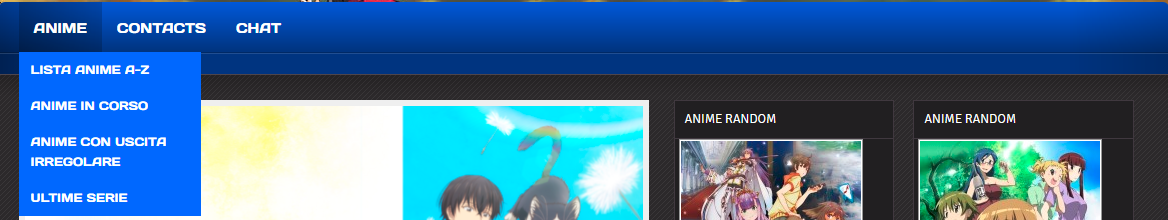
\includegraphics[width=1\textwidth]{img/menu.png}
	\caption{Menù} 
	\label{img4} 
\end{figure}